\documentclass[11pt,a4paper]{article}
\usepackage[a4paper,margin=1in]{geometry}
\usepackage[T1]{fontenc}
\usepackage[utf8]{inputenc}
\usepackage{lmodern}
\usepackage{amsmath,amssymb,amsthm,mathtools}
\usepackage{graphicx}
\usepackage{booktabs}
\usepackage{array}
\usepackage{microtype}
\usepackage{xcolor}
\usepackage{hyperref}
\usepackage[nameinlink,noabbrev]{cleveref}
\usepackage{enumitem}
\usepackage{authblk}
\usepackage[backend=biber,style=numeric,sorting=none,maxbibnames=99]{biblatex}
\addbibresource{refs.bib}
\hypersetup{colorlinks=true,linkcolor=blue!55!black,citecolor=blue!55!black,urlcolor=blue!55!black}
\graphicspath{{figures/}}
\newtheorem{proposition}{Proposition}
\newtheorem{lemma}{Lemma}
\newtheorem{remark}{Remark}
\newcommand{\psucc}{P_{\mathrm{succ}}}
\newcommand{\cl}{C_{\ell_1}}
\newcommand{\ord}{\mathrm{ord}}
\newcommand{\Tr}{\mathrm{Tr}}

\title{Minimal quotients for the SHIFT/Lugano causal witness}
\author[1]{Dmitry Alexandrovich Lugin}
\affil[1]{Independent researcher (no institutional affiliation)}
\date{Preprint draft; May 11, 2026\\DOI: \href{https://doi.org/10.5281/zenodo.20128994}{10.5281/zenodo.20128994}}

\begin{document}
\maketitle

\begin{abstract}
The SHIFT measurement is an eight-outcome product-basis measurement which, through its correspondence with the Lugano process, gives an operational benchmark for causal nonseparability.  We isolate a simple structural feature of this benchmark.  Let $L$ denote the eight-valued SHIFT label and let $C=f(L)$ be the four-valued Lugano output class obtained by applying $f(0)=f(1)=0$ and $f(+)=f(-)=1$ componentwise.  We prove that any stochastic coarse-graining of the SHIFT outcome to at most $m$ outcomes has optimal Lugano decoding success at most $\min(m,4)/4$.  Hence any coarse-graining with at most three outcomes cannot violate the Lugano causal bound $3/4$, whereas the four-outcome quotient $Y=f(L)$ reaches unit success.  Thus full eight-outcome SHIFT resolution is not operationally necessary; preserving the four Lugano quotient classes is necessary and sufficient for perfect success.

We use this quotient result to sharpen a record-based view of causal-order coherence.  Physical records do not merely reduce a scalar visibility; they preserve or destroy specific operational equivalence classes.  We formulate this with record Gram matrices acting as Schur dephasing maps on an effective order degree of freedom, prove monotonicity of $\ell_1$ order coherence under such record channels, and show by exhaustive enumeration of all $4140$ deterministic partitions of the SHIFT labels that outcome topology, not just the number of outcomes or a scalar coherence, determines whether the Lugano witness survives.  We also state limitations: cyclic precedence boxes are useful falsifiers of linear-order models but are not operational processes by themselves; the AF-BW/Lugano process is operational and logically consistent but signalling in the compressed input-output representation; and in a one-shot binary channel full parity erasure collapses to input-output independence.  These results position the proposed framework as a reproducible diagnostic of record topology in causal-nonseparability witnesses rather than as a claim of new fundamental noncausality.
\end{abstract}


\section{Scope and main claims}
\label{sec:scope}

Processes with indefinite causal order are a central test bed for the relation between quantum theory, information, and causality.  The quantum switch and process-matrix frameworks show that, in suitable operational settings, the temporal order of operations need not be represented by one fixed classical order \cite{Chiribella2009,Oreshkov2012,Araujo2015}.  At the same time, recent work emphasizes that one must distinguish different notions: causal nonseparability, noncausal correlations, signalling process functions, and operationally valid higher-order processes are not interchangeable \cite{KunjwalBaumeler2023,Steffinlongo2025,LiuOreshkov2025}.

This manuscript focuses on a narrow question which arose in our attempts to formalize ``records of causal order'': when an operational witness of indefinite causal order is implemented through a measurement with several possible outcomes, which part of the outcome information is actually needed to witness causal nonseparability?  For the SHIFT/Lugano benchmark, the answer is especially clean.  The full SHIFT measurement has eight labels, but the Lugano witness only depends on a four-valued quotient of these labels.  We prove that this quotient is minimal.

The paper has three levels of results.
\begin{enumerate}[leftmargin=2em]
    \item \textbf{Operational quotient theorem.}  Any stochastic coarse-graining of the eight SHIFT labels to $m\le 3$ outcomes has Lugano success at most $3/4$; the four-outcome quotient induced by $f(0)=f(1)=0$, $f(+)=f(-)=1$ reaches success $1$.  This is the main result of the paper.
    \item \textbf{Record topology.}  A physical record or coarse-graining preserves a witness only if it preserves the relevant quotient structure.  This gives a concrete operational meaning to the phrase ``record topology'', stronger than a scalar visibility.
    \item \textbf{Boundaries and limitations.}  We relate the quotient picture to Schur dephasing of order-coherence matrices, cyclic precedence witnesses, AF-BW/Lugano process functions, and parity erasure.  These parts are deliberately conservative: they identify useful diagnostics and no-go boundaries, not new physical processes.
\end{enumerate}

\paragraph{What is not claimed.}
We do not claim to discover the SHIFT measurement, the Lugano process, the quantum switch, or the fact that records suppress interference.  These are existing ideas.  The new contribution is the minimal quotient theorem for the SHIFT/Lugano witness, together with a record-topology interpretation and reproducible numerical checks.  We also do not claim a loophole-free or device-independent verification protocol; our analysis is a theoretical and computational diagnostic.

\section{The Lugano benchmark and the SHIFT measurement}
\label{sec:lugano}

The Lugano task uses three binary inputs $a,b,c\in\{0,1\}$ and asks for three binary outputs
\begin{equation}
    w_L(a,b,c)=(x,y,z)=\big(c(b\oplus1),\,a(c\oplus1),\,b(a\oplus1)\big).
    \label{eq:lugano}
\end{equation}
In the standard causal inequality for this task, causal strategies satisfy $\psucc\le 3/4$, whereas the Lugano process reaches $\psucc=1$ \cite{KunjwalBaumeler2023,Steffinlongo2025}.  Importantly, recent work shows that a quantum switch of classical communications can implement the SHIFT measurement and thereby simulate the structure of the Lugano process in a quantum-input scenario.  The successful SHIFT discrimination should therefore be read as a witness of causal nonseparability, not automatically as proof of fundamental noncausality \cite{Steffinlongo2025}.

The SHIFT basis is the eight-state product basis
\begin{equation}
\begin{split}
    \mathcal S=\{&|000\rangle, |+01\rangle, |01+\rangle, |01-\rangle,\\
                 &|1+0\rangle, |-01\rangle, |1-0\rangle, |111\rangle\}.
\end{split}
\label{eq:shiftbasis}
\end{equation}
where $|\pm\rangle=(|0\rangle\pm|1\rangle)/\sqrt2$.  Define the componentwise map
\begin{equation}
    f(0)=f(1)=0,\qquad f(+)=f(-)=1.
    \label{eq:fmap}
\end{equation}
For a SHIFT label $L=(\ell_1,\ell_2,\ell_3)$, the induced Lugano output class is
\begin{equation}
    C=f(L)=\big(f(\ell_1),f(\ell_2),f(\ell_3)\big).
\end{equation}
A direct calculation gives that, for a uniformly distributed computational input $|abc\rangle$, measuring in the SHIFT basis and applying $f$ reproduces \eqref{eq:lugano} with probability one.  Numerically, the Gram matrix of \eqref{eq:shiftbasis} differs from the identity by at most $2.2\times10^{-16}$, and the success probability is one for all eight inputs.

\begin{figure}[t]
    \centering
    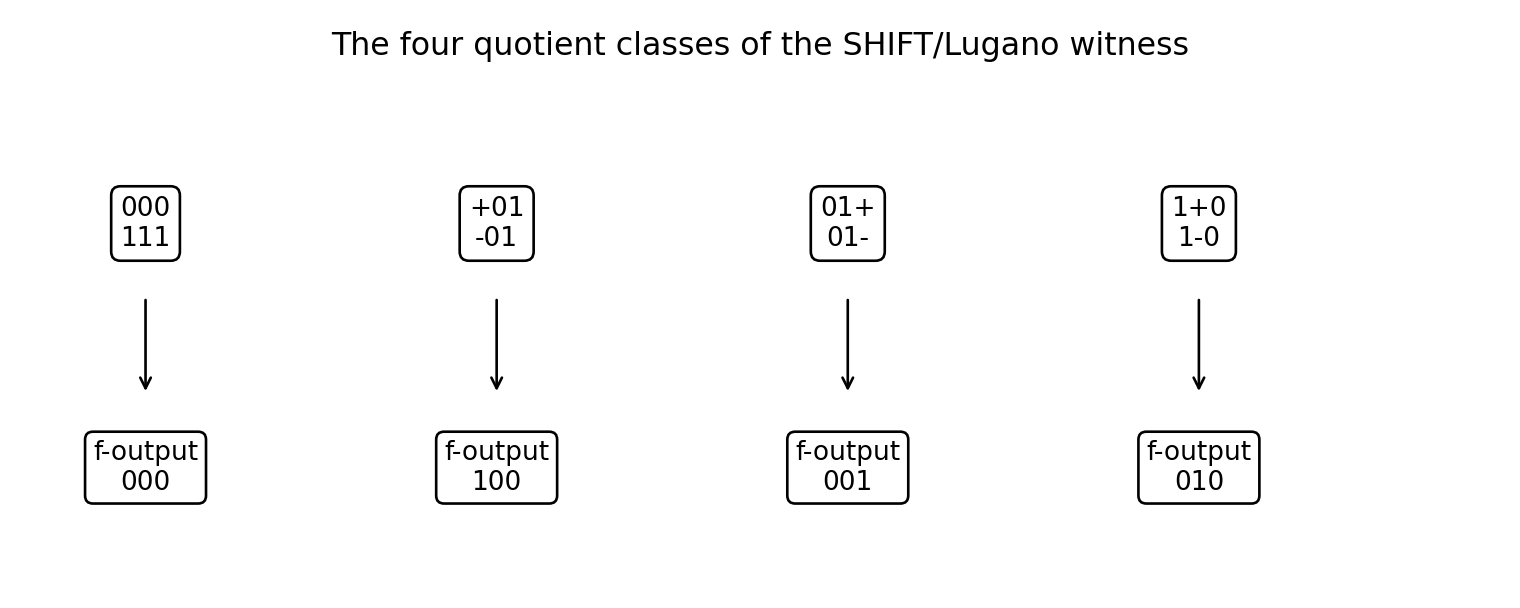
\includegraphics[width=0.82\linewidth]{fig_shift_quotient_diagram.png}
    \caption{The four-outcome quotient of the eight SHIFT labels.  The Lugano task does not require distinguishing all eight labels.  It only requires distinguishing the four classes induced by $C=f(L)$: $\{000,111\}$, $\{+01,-01\}$, $\{01+,01-\}$, and $\{1+0,1-0\}$.}
    \label{fig:quotient-diagram}
\end{figure}

\subsection{Reproducing the causal bound}
\label{subsec:causalbound}

A fixed total order is too restrictive for the Lugano causal inequality.  If we brute-force deterministic fixed total orders, allowing later parties to learn earlier inputs, the best success is $5/8$.  The standard causal inequality allows a dynamic causal strategy: one party is first, and the order of the remaining two parties may depend on the first party's local information.  Enumerating deterministic strategies of this form gives the expected bound $3/4$ for each possible first party, as shown in \cref{fig:dynamic-bound}.

\begin{figure}[t]
    \centering
    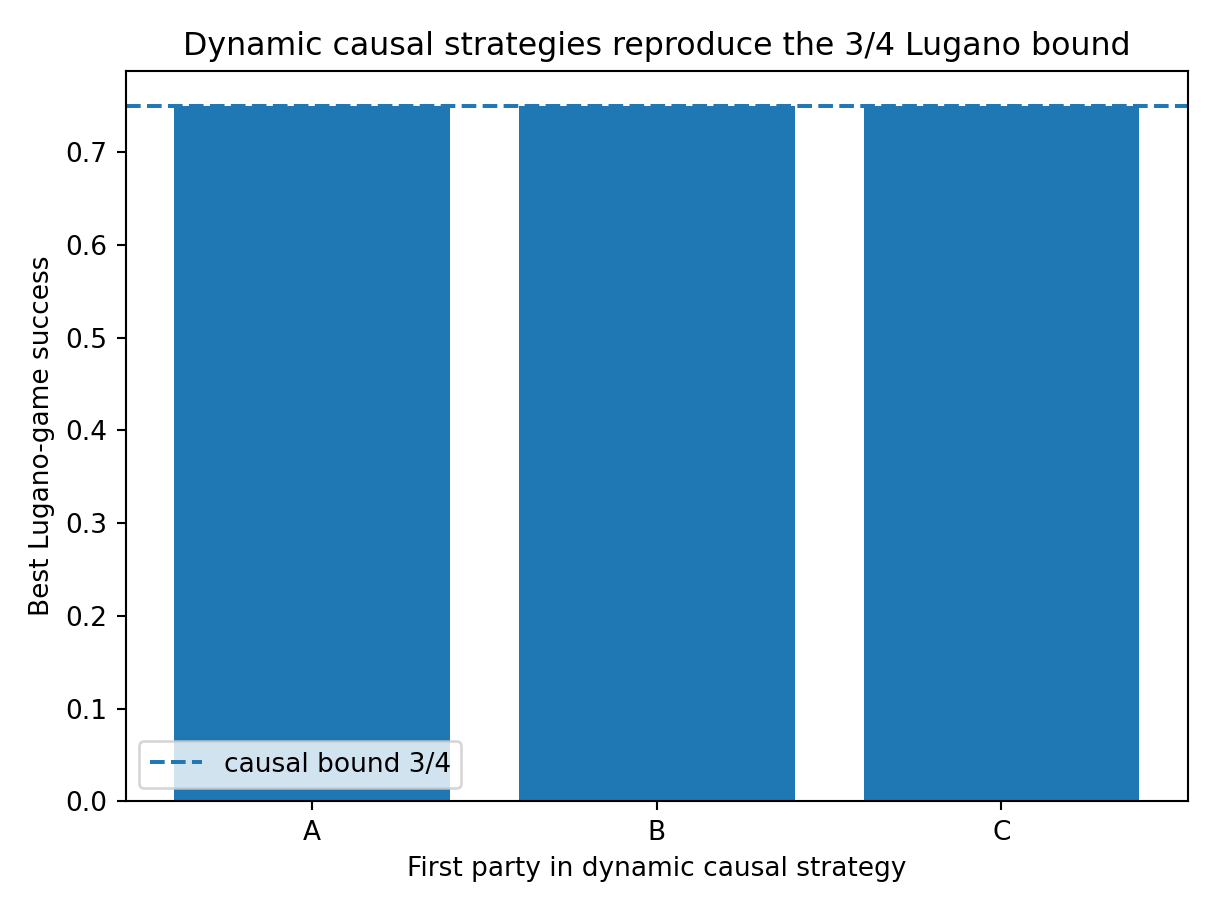
\includegraphics[width=0.7\linewidth]{fig_dynamic_bound.png}
    \caption{Brute-force verification of the Lugano causal bound.  Dynamic causal strategies with one first party reach $3/4$, reproducing the standard causal inequality.  Fixed total orders are more restrictive and reach only $5/8$ in the model used here.}
    \label{fig:dynamic-bound}
\end{figure}

\section{Minimal quotient theorem}
\label{sec:theorem}

We now prove the central result.  The theorem is stated for arbitrary stochastic coarse-grainings, so deterministic partitions are included as a special case.

\begin{proposition}[Minimal quotient for the SHIFT/Lugano witness]
\label{prop:minimalquotient}
Let $L$ denote the eight-valued outcome of the SHIFT measurement and let $C=f(L)$ denote the four-valued Lugano output class obtained by applying \eqref{eq:fmap} componentwise.  For uniformly distributed computational inputs, $C$ is uniformly distributed over four values and equals the Lugano target $w_L(a,b,c)$ with probability one.

Let $Y$ be any coarse-grained outcome obtained from $L$ by an arbitrary stochastic channel $P(Y|L)$, with $|Y|\le m$.  Then the optimal decoding success probability satisfies
\begin{equation}
    \psucc\le \frac{\min(m,4)}{4}.
    \label{eq:quotientbound}
\end{equation}
In particular, any coarse-graining with at most three outcomes cannot violate the Lugano causal bound $3/4$, whereas the four-outcome quotient $Y=C=f(L)$ achieves $\psucc=1$.
\end{proposition}

\begin{proof}
For a decoder $d:Y\to\{1,2,3,4\}$,
\begin{equation}
    \psucc=\sum_y P(Y=y,C=d(y)).
\end{equation}
The optimal decoder chooses, for each $y$, a class $c_y$ maximizing $P(Y=y,C=c)$, hence
\begin{equation}
    \psucc=\sum_y \max_c P(Y=y,C=c)=\sum_y P(Y=y,C=c_y).
\end{equation}
Grouping terms by $c_y$ gives
\begin{equation}
    \psucc=\sum_c\sum_{y:c_y=c}P(Y=y,C=c)
    \le \sum_{c\in\{c_y:y\in Y\}}P(C=c).
\end{equation}
At most $m$ classes appear in the last sum, and $P(C=c)=1/4$ for each of the four Lugano classes.  Thus $\psucc\le m/4$ for $m\le4$, and the trivial upper bound $1$ applies for $m\ge4$.  The bound is achieved by assigning one outcome to each of $m$ classes.  In particular, the four-outcome quotient $Y=f(L)$ preserves the Lugano target exactly and reaches $\psucc=1$.
\end{proof}

This proposition identifies the operational content of the SHIFT measurement for the Lugano witness.  Full eight-label resolution is unnecessary; the relevant resource is preservation of the four quotient classes.

\begin{figure}[t]
    \centering
    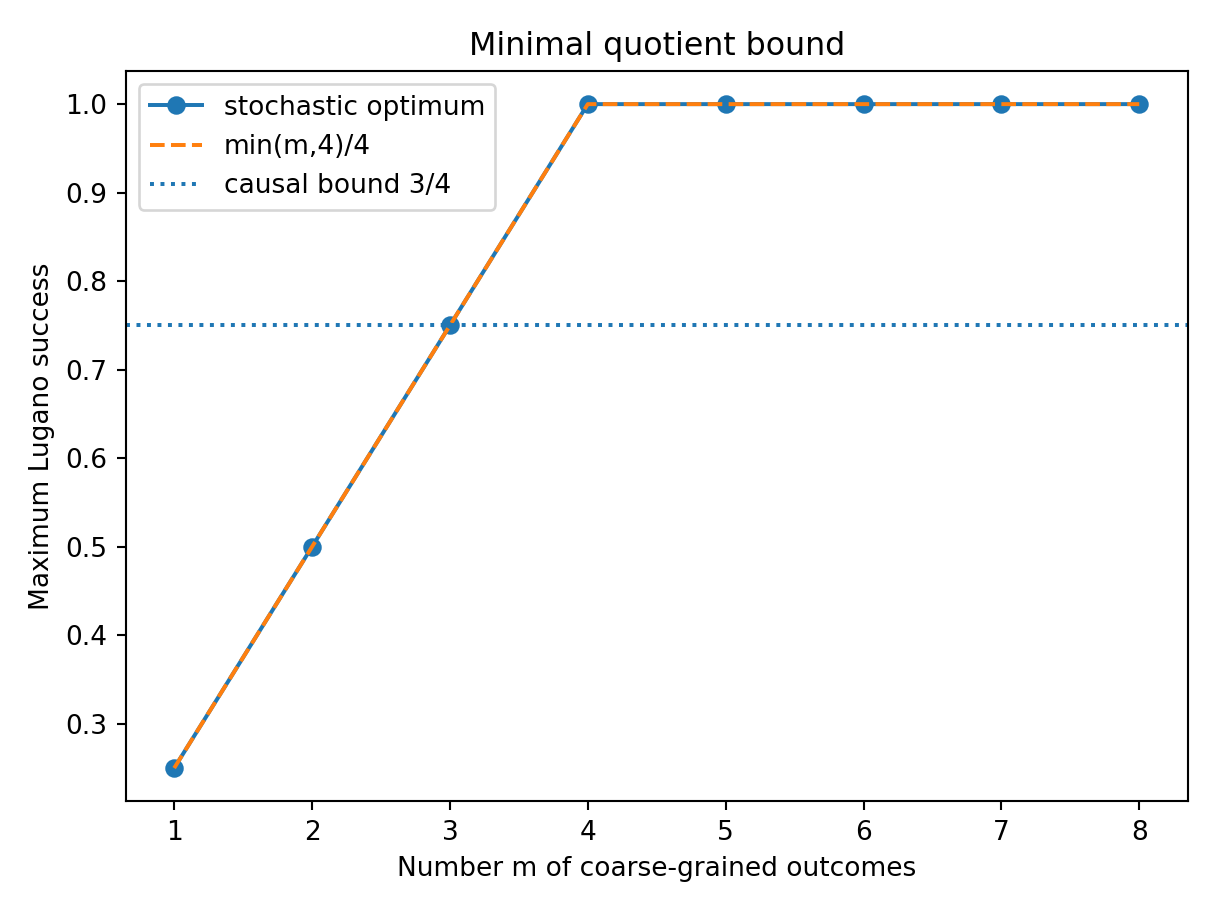
\includegraphics[width=0.72\linewidth]{fig_quotient_bound.png}
    \caption{The stochastic coarse-graining optimum of \cref{prop:minimalquotient}.  With $m\le3$ outcomes the best success is at most $3/4$, so the Lugano causal bound cannot be violated.  The four-outcome quotient $Y=f(L)$ reaches unit success.}
    \label{fig:quotient-bound}
\end{figure}

\section{All deterministic partitions of the SHIFT outcomes}
\label{sec:partitions}

To check the theorem and to understand the structure of deterministic coarse-grainings, we enumerated all set partitions of the eight SHIFT labels.  There are $4140$ such partitions.  For each partition we computed the best decoder from coarse-grained outcomes to Lugano outputs.  The numerical results match the theorem exactly: one, two, and three blocks reach at most $1/4$, $1/2$, and $3/4$ respectively; four blocks can reach one.

\begin{figure}[t]
    \centering
    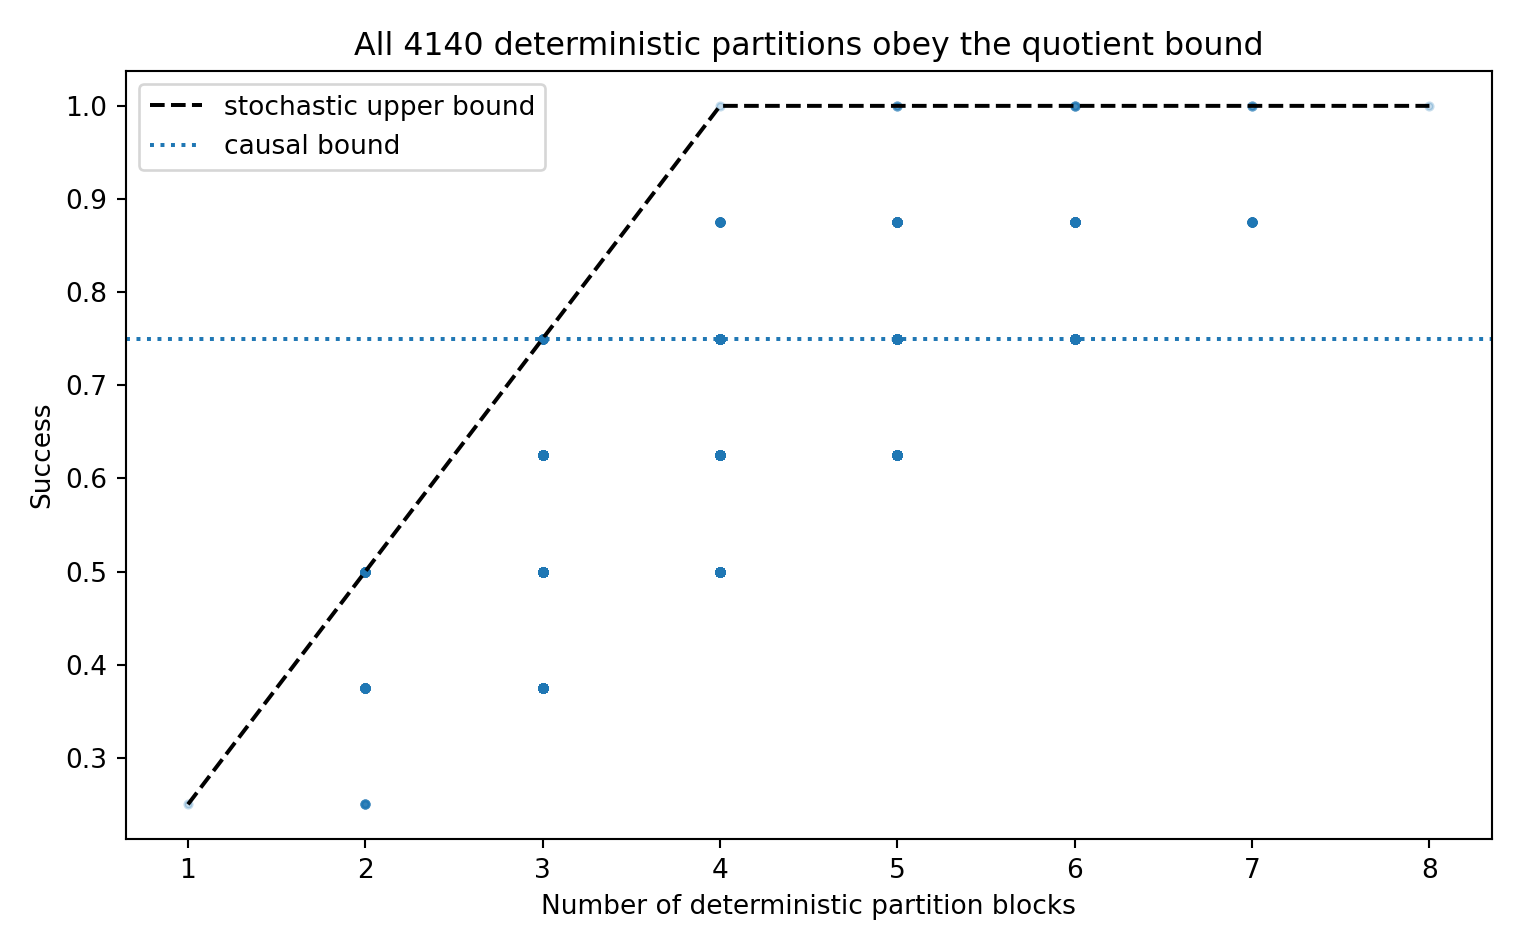
\includegraphics[width=0.78\linewidth]{fig_all_partitions.png}
    \caption{All $4140$ deterministic partitions of the eight SHIFT labels.  No partition with at most three blocks violates $3/4$.  Perfect success occurs exactly when the partition refines the four-class quotient induced by $f(L)$.}
    \label{fig:all-partitions}
\end{figure}

A particularly important partition is
\begin{equation}
\begin{split}
    \{000,111\},\qquad \{+01,-01\},\\
    \{01+,01-\},\qquad \{1+0,1-0\}.
\end{split}
\label{eq:fpartition}
\end{equation}
This partition has only four outcomes but reaches perfect Lugano success.  In the exhaustive enumeration, perfect deterministic partitions are exactly those which refine \eqref{eq:fpartition}: they may split a quotient class further, but they never mix labels belonging to different $f$-output classes.

\begin{remark}[Why this is not a scalar visibility statement]
The number of outcomes, or a scalar measure such as partition entropy, does not determine the witness value.  The operational question is whether a record preserves the quotient structure relevant to the task.  A coarse-graining that forgets distinctions inside a quotient class is harmless; a coarse-graining that mixes quotient classes can destroy the witness.
\end{remark}

\section{Record topology and robust quotient preservation}
\label{sec:recordtopology}

A physical measurement record can be modeled as a noisy or partial readout of the ideal SHIFT label.  We therefore interpret the quotient theorem as a statement about record topology: a record can be incomplete but still operationally sufficient if it preserves the $f$-quotient.

We simulated a simple confusion model.  A partition $\Pi$ of the eight labels defines blocks.  With probability $\eta$, the reported label is the true label; with probability $1-\eta$, it is uniformly randomized inside the same block.  If the blocks are the four $f$-classes, this internal confusion does not affect the Lugano output at all.  By contrast, one-block or two-block coarse-grainings must retain a sufficiently large identity component to exceed $3/4$.

\begin{figure}[t]
    \centering
    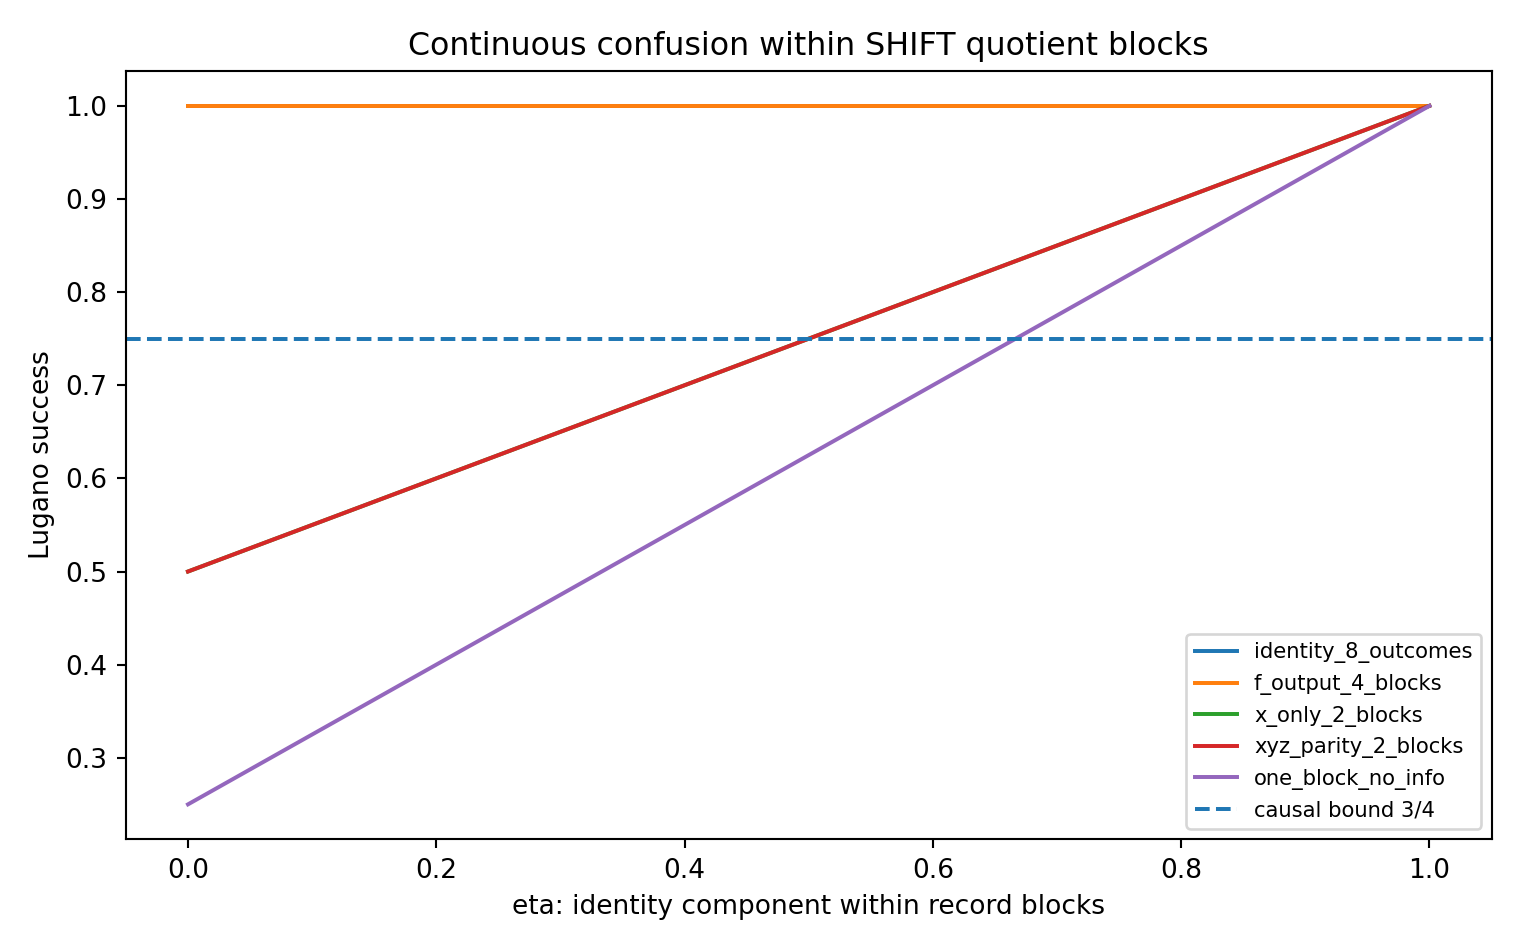
\includegraphics[width=0.82\linewidth]{fig_continuous_confusion.png}
    \caption{Continuous confusion within coarse-grained SHIFT-label blocks.  The four $f$-output blocks preserve the Lugano witness for all values of the within-block confusion parameter.  Coarse-grainings that mix different Lugano quotient classes require a high identity component and can fail to violate the $3/4$ bound.}
    \label{fig:confusion}
\end{figure}

This gives a concrete operational version of our earlier record-graph intuition.  A record is not merely ``strong'' or ``weak''.  It can be strong in an irrelevant direction and weak in a relevant one.  For a given witness, the relevant information is the quotient structure that the witness reads.

\subsection{Schur record channels}
\label{subsec:schur}

The same idea can be written in a more abstract order-coherence notation.  Let $\rho_{ij}$ be an effective coherence matrix over alternative labels or orders, and let $\Gamma_{ij}=\langle R_j|R_i\rangle$ be the Gram matrix of the record states.  Tracing over the record induces the Schur channel
\begin{equation}
    \rho\mapsto \rho\circ\Gamma,
    \label{eq:schur}
\end{equation}
where $\circ$ is entrywise multiplication.  Since $\Gamma$ is a correlation matrix, $|\Gamma_{ij}|\le1$, and therefore
\begin{equation}
    \cl(\rho\circ\Gamma)
    =\sum_{i\ne j}|\rho_{ij}\Gamma_{ij}|
    \le \sum_{i\ne j}|\rho_{ij}|=\cl(\rho).
    \label{eq:l1monotone}
\end{equation}
This is a simple coherence monotonicity statement, not a new measurement theory.  Its relevance here is that it keeps track of \emph{which} edges of a record graph survive, not only how much scalar coherence remains.

\subsection{Same scalar coherence, different witness behavior}
\label{subsec:samescalar}

To illustrate why topology matters, we compared two record matrices with the same normalized off-diagonal $\ell_1$ coherence, $\cl=0.4$, but different block structures.  One preserves a parity-like mode; the other preserves a different pairing structure.  In a simple Lugano-like mode model, both can preserve a uniform mode, but only one preserves the parity mode.  Thus the same scalar coherence can correspond to different witness survival.

\begin{figure}[t]
    \centering
    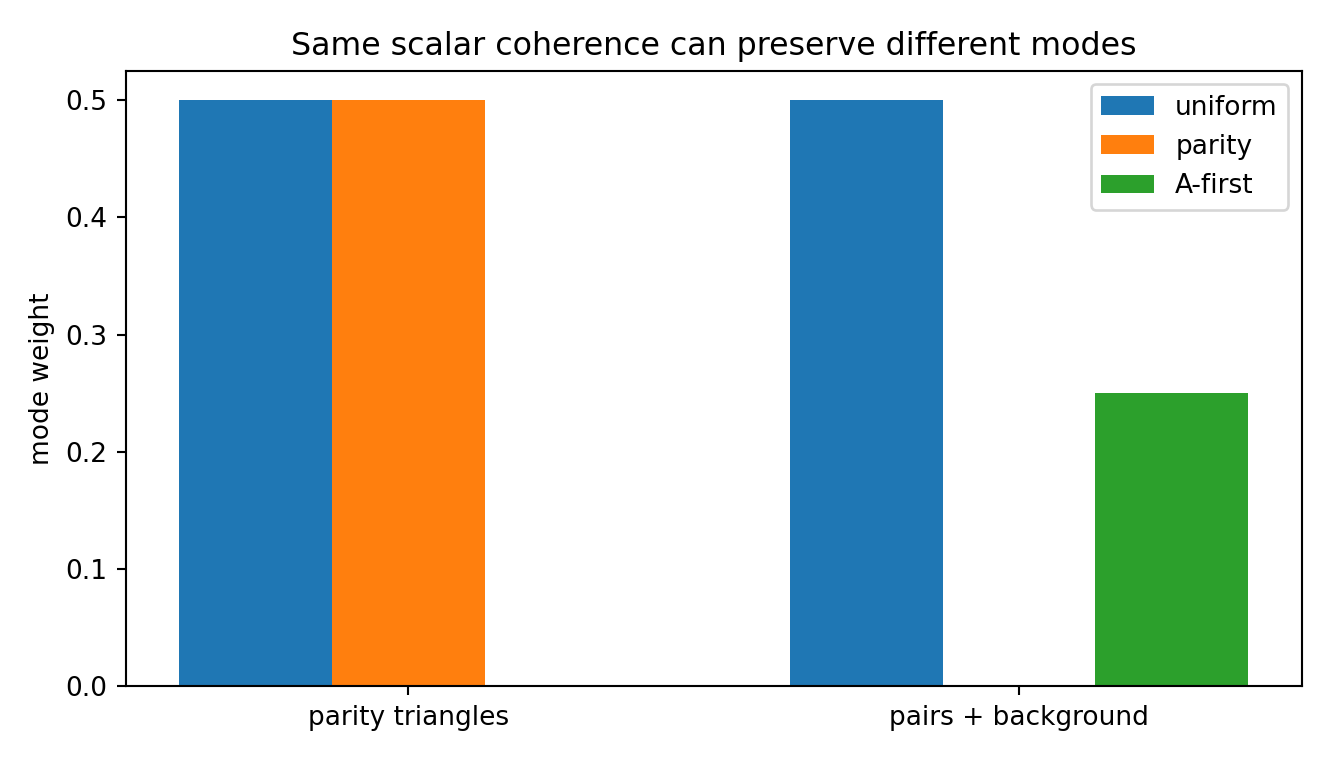
\includegraphics[width=0.82\linewidth]{fig_topology_witness.png}
    \caption{Two record topologies with the same scalar coherence can support different causal-mode diagnostics.  This motivates using record topology or quotient preservation rather than a single visibility parameter.  The plotted witness-success model is diagnostic rather than a full process-matrix derivation.}
    \label{fig:topology}
\end{figure}

\section{Cyclic witnesses, AF-BW, and parity-erasure boundaries}
\label{sec:boundaries}

The quotient result concerns the SHIFT/Lugano witness.  It should not be conflated with stronger claims about cyclic causality.  In earlier exploratory calculations we also studied cyclic precedence boxes and the AF-BW/Lugano process function.

For three events, any mixture of linear orders obeys
\begin{equation}
    1\le P(A<B)+P(B<C)+P(C<A)\le2.
    \label{eq:cyclebound}
\end{equation}
A box violating \eqref{eq:cyclebound} is a useful falsifier of a linear-order model.  However, a no-signalling cyclic precedence box can be operationally trivial: it can output order facts independently of local choices.  Conversely, the AF-BW process function is operational and logically consistent, but it is signalling in the compressed input-output representation \cite{BaumelerWolf2016,KunjwalBaumeler2023}.  This is why we do not identify cyclic order facts with a physical noncausal process.

Parity erasure gives a further boundary.  Liu and Oreshkov recently proposed parity erasure as a foundational principle characterizing processes with indefinite causal order in a locally sequential framework \cite{LiuOreshkov2025}.  In the simplified one-shot binary channel $W(I|O)$ used in our exploratory checks, a Walsh-Fourier decomposition shows that erasing all nonempty parity components forces $W(I|O)$ to be independent of $O$.  This explains why a compressed CPB/AF-BW bridge is hard: full parity erasure removes the very operational dependence that would make the box nontrivial.  This observation is only a boundary result in the compressed model, not a no-go theorem for the full higher-order process framework.

\section{Reproducibility and numerical checks}
\label{sec:reproducibility}

All numerical statements in this manuscript are generated by short Python scripts.  The main checks are:
\begin{itemize}[leftmargin=2em]
    \item enumeration of dynamic deterministic causal strategies for the Lugano bound $3/4$;
    \item verification that the SHIFT basis is orthonormal and that $f(L)$ reproduces $w_L(a,b,c)$ on computational inputs;
    \item proof-level computation of the stochastic quotient bound $\min(m,4)/4$;
    \item exhaustive enumeration of all $4140$ deterministic partitions of the eight SHIFT labels;
    \item confusion-model simulations for named coarse-grainings;
    \item record-matrix diagnostics illustrating scalar-coherence insufficiency.
\end{itemize}
The scripts, CSV outputs, and figure-generation workflow needed to reproduce the numerical checks in this manuscript are available in the \href{https://github.com/bringmetheural/minimal-shift-lugano-quotients}{GitHub repository}.  The archived release is available through \href{https://doi.org/10.5281/zenodo.20128994}{Zenodo}.

\section{Discussion}
\label{sec:discussion}

The main lesson is simple but operationally precise.  In the SHIFT/Lugano benchmark, the relevant resource is not full eight-outcome resolution of the SHIFT label.  The relevant resource is preservation of the four-valued quotient $f(L)$.  This quotient is necessary and sufficient for perfect Lugano success, and three or fewer outcomes cannot violate the causal bound.

This result also refines the broader ``record of causal order'' intuition.  A record does not have to preserve all microscopic alternatives.  It has to preserve the quotient structure read by the witness.  Therefore, record topology is an operational object: two records with similar scalar coherence can behave differently if they preserve different quotient classes.

Several limitations should remain explicit.  First, the quotient theorem is about the SHIFT/Lugano witness, not a universal theorem about all causal-nonseparability witnesses.  Second, the record-matrix and Schur-channel framework is an effective description of record-induced dephasing; it is not, by itself, a full process-matrix embedding.  Third, the cyclic precedence and parity-erasure discussions are boundary diagnostics, not claims of a new noncausal process.  These limitations are important because the current literature carefully distinguishes causal nonseparability, noncausal correlations, process functions without global past, and device-independent tests of indefinite causal order \cite{Oreshkov2012,Araujo2015,KunjwalBaumeler2023,Steffinlongo2025,LiuOreshkov2025,Valibouse2026}.

\section{Conclusion}

We have shown that the SHIFT/Lugano witness admits a minimal quotient structure.  Any coarse-graining of the eight SHIFT outcomes to at most three outcomes cannot violate the Lugano causal bound $3/4$.  A four-outcome quotient, obtained by applying $f(0)=f(1)=0$ and $f(+)=f(-)=1$ componentwise to the SHIFT label, reaches unit success.  The theorem is independent of whether the coarse-graining is deterministic or stochastic.

This gives a concrete, operationally anchored version of record topology: a record preserves a causal-nonseparability witness when it preserves the quotient classes used by that witness.  The result turns the earlier abstract idea of causal-order coherence graphs into a testable statement about partial measurements in the SHIFT/Lugano benchmark.  The remaining open direction is to embed this quotient-topology analysis directly into the process-matrix or distributed-measurement formalism of quantum switches, and to characterize analogous minimal quotients for broader families of causally nonseparable measurements.

\paragraph{Acknowledgements.} The author reports no institutional affiliation and no external funding for this work.


\appendix

\section{Dynamic causal strategies for the Lugano bound}
\label{app:causal-bound}

This appendix spells out the finite deterministic check used in \cref{subsec:causalbound}.  The Lugano target is
\begin{equation}
    w_L(a,b,c)=\big(c(b\oplus1),\,a(c\oplus1),\,b(a\oplus1)\big).
\end{equation}
A fixed total order is more restrictive than the standard causal model for this inequality.  In a fixed total order, the first party can depend only on its own input, the second party can depend on the first party's input and its own input, and the last party can depend on all inputs.  Exhaustive enumeration of deterministic strategies in this restricted model gives success $5/8$ for every fixed order.

For the causal inequality, the relevant deterministic causal strategy is dynamic.  One party is first.  Its output depends only on its own input.  Conditional on the first party's local information, the ordering of the remaining two parties may be chosen.  The second party can use its own input and the first party's local information, and the last party can use all inputs.  Enumerating these deterministic strategies gives six successes out of eight uniformly distributed inputs, i.e. $3/4$, independently of which party is first.  Since shared randomness only convexly mixes deterministic strategies, it cannot exceed the deterministic maximum.

\begin{center}
\begin{tabular}{lcc}
\toprule
Model & best successes out of 8 & success probability\\
\midrule
Fixed total order & 5 & $5/8$\\
Dynamic causal strategy & 6 & $3/4$\\
Ideal SHIFT/Lugano & 8 & $1$\\
\bottomrule
\end{tabular}
\end{center}

\section{Exhaustive partition check}
\label{app:partition-check}

The proof of \cref{prop:minimalquotient} applies to arbitrary stochastic coarse-grainings.  As a finite sanity check, we also enumerated all set partitions of the eight SHIFT labels.  There are $B_8=4140$ such partitions, where $B_8$ is the eighth Bell number.  For each partition, we computed the optimal decoder from blocks to the four Lugano output classes.

\begin{center}
\begin{tabular}{rrrrrr}
\toprule
Blocks & count & min success & max success & violating & perfect\\
\midrule
1 & 1 & $1/4$ & $1/4$ & 0 & 0\\
2 & 127 & $1/4$ & $1/2$ & 0 & 0\\
3 & 966 & $3/8$ & $3/4$ & 0 & 0\\
4 & 1701 & $1/2$ & $1$ & 25 & 1\\
5 & 1050 & $5/8$ & $1$ & 76 & 4\\
6 & 266 & $3/4$ & $1$ & 78 & 6\\
7 & 28 & $7/8$ & $1$ & 28 & 4\\
8 & 1 & $1$ & $1$ & 1 & 1\\
\bottomrule
\end{tabular}
\end{center}

The enumeration also verifies the equality condition for perfect deterministic coarse-grainings: a partition reaches success $1$ if and only if it refines the four-class quotient $f(L)$.  Thus perfect success does not require resolving all eight SHIFT labels, but it does require never mixing labels belonging to different Lugano output classes.

\section{Source package and arXiv-ready files}
\label{app:source-package}

The source package contains the \LaTeX{} manuscript, bibliography, figures, and Python scripts used to reproduce the main tables and figures.  For arXiv submission, the preferred upload is the \LaTeX{} source archive rather than a PDF generated from \LaTeX{}.  The repository archive accompanying this manuscript is intentionally kept small and excludes intermediate render logs, rendered page images, and unrelated scratch files.  The scripts regenerate the CSV tables and figures used in the paper from the definitions of the Lugano map and the SHIFT basis.


\printbibliography

\end{document}
